\chapter{Prozesserstellungsversuche}
Der Architekturprozess ist komplex und ein falsches Vorgehen kann der Ursprung vieler Probleme sein \cite[S. 7-8]{softarch}. Deswegen ist es notwendig einen eigenen Prozess zu definieren, welcher die Erstellung vereinfacht und die Fehlerkosten minimiert. Dieser Prozess sollte schon in der Planungsphase zum Einsatz kommen, da hier wegen der Zehner-Regel der Fehlerkosten der größte Effekt zur Reduzierung der Fehlerkosten erzielt werden kann \cite[S. 154]{fehler}.

Der Prozess wurde anhand eines Beispielprojektes erstellt und dreht sich um die Architektur eines Systems einer Personenzertifizierungsstelle.

\section{Vorhandene Daten}
Ausgegangen wurde von folgenden Anforderungsdokumenten, welche in der Erstellung des Prozesses mehrfach abgeändert und an die Architekturprozessanforderungen angepasst wurden:

\begin{itemize}
  \item Usecasediagramm: modelliert die Usecases des Unternehmens
  \item Usecasebeschreibung: ausgefülltes Anforderungstemplate, welches Sonderfälle, nicht funktionale Parameter und weitere Details beinhaltet
  \item Klassendiagramm: visualisiert die zu verwendeten Daten
  \item Aktivitätsdiagramme: visualisiert den Ablauf komplexerer Usecases
  \item Kontextdiagramm: zeigt die Datenflüsse zwischen AkteurInnen, Nachbarsystemen und dem zu erstellenden System
  \item ISO Anforderungsdokument für Personenzertifizierungsstellen \cite{ISO_CERT}: beschreibt die Rahmenbedingungen für den Betrieb einer Personenzertifizierungsstelle
\end{itemize}

\section{Prozesserstellungsversuche}
Ausgehend von den vorhandenen Daten wurden mehrere Prozesse definiert, welche bis auf den Letzten entweder zu grobe Ergebnisse lieferten, oder nicht nachvollziehbar waren.

Ausgangsbasis war eine Systemvision mit folgenden Anforderungen:

\begin{itemize}
  \item Es soll eine Webseite entstehen, welche die Prüfungstermine auflistet und Personen erlaubt, sich für diese Prüfungen anzumelden. Dadurch soll der Verwaltungsaufwand reduziert werden, um Kosten zu sparen.
  \item Die Übermittlung der Prüfungsdaten soll über einen eigenen VPN Server geschehen, um die Datensicherheit des Systems zu erhöhen.
  \item Die Prüfungsdaten werden firmenintern verwaltet und nach der Auswertung soll der Scheme Owner benachrichtigt werden. Beide Usecases sollen auf eine sichere Art und Weise umgesetzt werden.
\end{itemize}

\begin{figure}[!htbp]
    \centering
    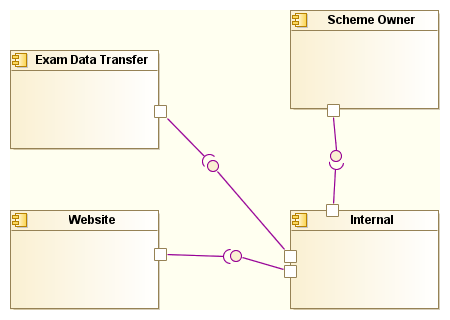
\includegraphics[scale=0.6]{uml/vision.png}
    \caption{Systemvision der Komponenten}
\end{figure}

Aufbauend darauf wurde dann versucht einen Prozess zu finden, der diese Grundideen berücksichtigt.

Die anfänglichen Versuche basierten stark auf einem ATAM Utility Tree ähnlichen Verfahren, bei welchem die nicht funktionalen Anforderungen nach der Formel von Oliver Vogel priorisiert wurden: \glqq Priorität = (Nutzen + Risiko + Wirkung) / 3\grqq \cite[S. 374]{softarch}. Die Bewertung der Komponenten wurde auf Basis einer bestehenden Tabelle mit Basisarchitekturen abgeleitet \cite[S. 179]{review}.


\subsection{Vom Usecase zur Komponente durch Priorisierung der nicht funktionalen Anforderungen}
Der erste Versuch zur Erstellung des Architekturprozesses orientierte sich am Prinzip: teile und herrsche. Der Prozess verwendete aufgrund der initialen Vermutung, dass nicht funktionalen Anforderungen die Hauptentscheidungsbasis für die Architektur darstellen, eine priorisierte Liste von nicht funktionalen Anforderungen. Danach wurde versucht, anhand der priorisierten Anforderungen passende Komponenten auszuwählen. Der genaue Ablauf war wie folgt:

\begin{itemize}
  \item Für jeden Usecase wird ein komplettes Komponentendiagramm des Systems erstellt.
  \item Die Komponenten jedes Teilsystems werden anhand ihrer nicht funktionalen Qualitäten aus einem Pool von Komponentenarchitekturen gewählt. Diese Komponentenarchitekturen beinhalteten zB. Systeme wie den üblichen Webstack, welcher sich aus Komponenten wie dem Loadbalancer, Datenbankserver, Applikationsserver und Webserver zusammensetzt.
  \item Schlussendlich werden alle Teilsysteme miteinander vereinigt, soweit es die nicht funktionalen Attribute erlauben.
\end{itemize}

Dieser Prozess scheiterte nicht nur am enormen Modellierungsaufwand, sondern auch am Auswahlprozess der Komponentenarchitekturen: Je nachdem, welche Komponentenarchitekturen vorhanden waren und wie diese bewertet wurden, entstanden unterschiedliche Architekturen. Zudem schien es zu viele Komponentenarchitekturen zu geben, da einzelnen Komponenten beliebig miteinander kombinierbar waren.

Die Qualität der Architektur hätte folglich von der Vollständigkeit dieser scheinbar unendlich großen Menge an Komponentenarchitekturen abgehangen. Aus diesem Grund schien der Prozess ungeeignet für die Architekturerstellung und wurde somit verworfen.

\subsection{Von einer Architektur mit hoher Kohäsion und anschließendem Architekturreview zu den Komponenten}
Um das Problem des sehr hohen Modellierungsaufwandes des ersten Prozesses zu umgehen, wurde von einer Grundarchitektur mit hoher Kohäsion ausgegangen. Diese Komponentenarchitektur entstand zusammen mit dem/der AuftraggeberIn, um zusätzliche Risiken indentifizieren zu können.

\begin{figure}[!htbp]
    \centering
    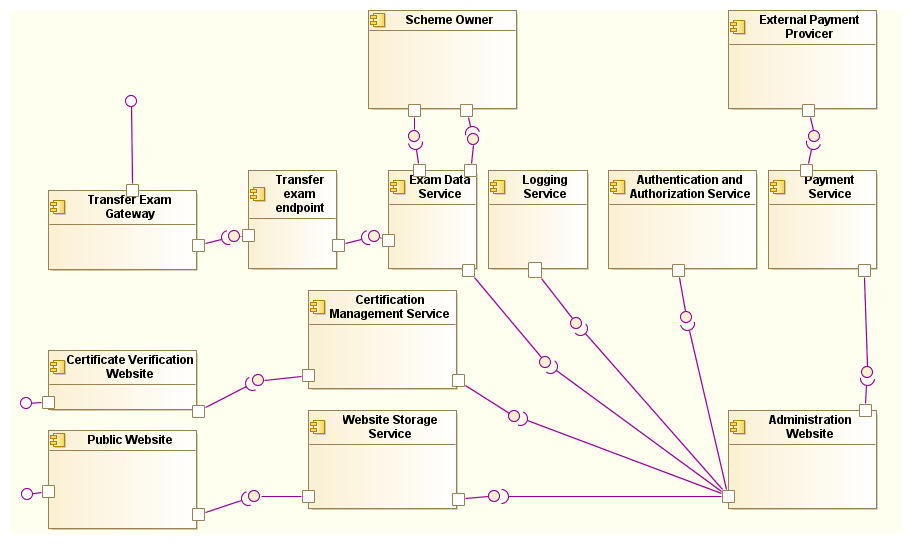
\includegraphics[scale=0.5]{uml/vision2.png}
    \caption{Architektur mit hoher Kohäsion}
\end{figure}

Diese Architektur sollte nun auf die Erfüllung der nicht funktionalen Anforderungen überprüft und gegebenenfalls angepasst werden. Zur Überprüfung der Anforderungen wurden die priorisierten, nicht funktionalen Anforderungen eines Usecases herangezogen. Der Prozess ähnelte damit stark einem szenariobasierten Review wie er zB. in ATAM durchgeführt wird.

Auch dieser Prozess litt jedoch unter dem Problem, dass die nicht funktionalen Anforderungen schwer bewertet werden konnten. Außerdem war es schwer ein Regelwerk/Rezept aus der Architekturerstellung abzuleiten, da durch die Einbeziehung unterschiedlicher AuftraggeberInnen jeweils verschiedene Architekturen entstehen können. Die Einbeziehung von Kohäsion als Aufteilungsgrundlage der Komponenten verursachte zudem ein gefühlt zu großes System, welches in der Umsetzung sehr teuer geworden wäre. Die Kostenersparnis des Systems, welche in der Systemvision definiert wurde, schien damit unzureichend erfüllt zu werden.

\subsection{Von den Daten zu den Komponenten}
Die Auswahl und Bewertung der Komponentenarchitekturen und der starke Fokus auf die nicht funktionalen Anforderungen in den beiden vorherigen Prozessen stellte ein wesentliches Hindernis zur Erstellung eines eindeutigen Regelwerkes dar: Eine vollständige Auflistung aller möglichen Komponentenarchitekturen erschien entweder unmöglich oder unvollständig zu sein; eine Bewertung der nicht funktionalen Attribute schien ohne entsprechende Implementation nur sehr grob überprüfbar zu sein. Der Versuch, ein System mit hoher Kohäsion zu erstellen, endete zudem in sehr teuren Architekturen.

Dies war überraschend, da die populärste Architekturbewertungsmethode, ATAM, stark auf nicht funktionale Anforderungen aufbaute. Als Grund für diese Inkompatibilität wurde der Zeitpunkt der Architekturerstellung vermutet: Durch die fehlende Implementationsphase waren die nicht funktionalen Anforderungen sehr schwer zu bewerten und somit mehr oder weniger nicht überprüfbar. Deshalb wurden sie als Hauptkriterium und Ausgangspunkt für die Architekturerstellung verworfen.

Stattdessen wurde der Fokus auf die Aufspaltung der Daten gelegt. Die Daten wurden anhand Ihrer Vertraulichkeit in unterschiedliche Netze aufgeteilt. Diese Netze wurden dann durch Komponenten miteinander verbunden, die den Zugriff auf die Daten regelten.

\begin{figure}[!htbp]
    \centering
    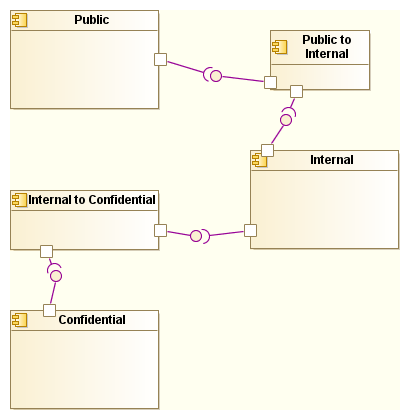
\includegraphics[scale=0.7]{uml/vision3.png}
    \caption{Aufteilung der Komponenten in Datenbereiche}
\end{figure}

Dieser Prozess erlaubte es, eine nachvollziehbare Architektur zu erstellen, jedoch war das Ergebnis zu grob. Außerdem schien eine separate Komponente zur  Übertragung der Prüfungsdaten zu fehlen, welche in der ursprünglichen Systemvision definiert und als notwendig empfunden worden war, um die Rahmenbedingungen der Vertrautheit zu erfüllen \cite[7.3]{ISO_CERT}.

\subsection{Von den Daten und den AkteurInnen zu den Komponenten}
Aufbauend auf dem vorherigen Prozess, welcher die Architektur anhand der Daten erstellte, wurden nun auch AkteurInnen eingebunden und deren Beziehungen zu den Daten ermittelt. Anhand dieser Beziehungen wurden Regeln erstellt, aus denen wiederum die Architektur erstellt wurde.

\begin{figure}[!htbp]
    \centering
    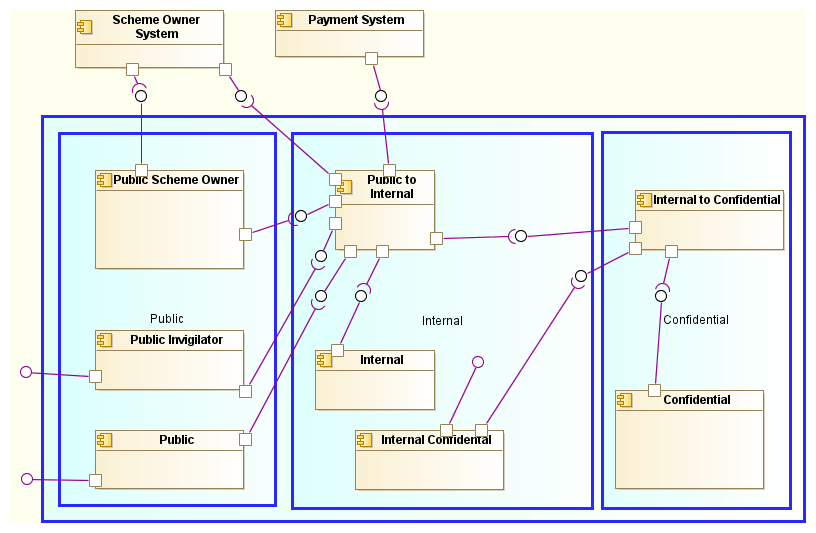
\includegraphics[scale=0.55]{uml/vision4.png}
    \caption{Aufteilung der Komponenten in Datenbereiche und AkteurInnen}
\end{figure}

Dieser Prozess schien nicht nur die Rahmenbedingungen und Sicherheitsbedingungen abzudecken, er war auch durch die erstellten Regeln nachvollziehbar und genau genug, um bereits einen guten Blick auf die Architektur zu erlangen. Anhand der daraus resultierenden Architektur war es nun auch möglich, nicht funktionale Attribute wie zB. Antwortzeiten besser einschätzen zu können.
